%! Author = sriadityavedantam
%! Date = 4/8/26

\section{Hypersurfaces}
Let $X\subset\pp^2$. In this section we want to describe the space of regular 1-forms $\Omega[X]$, when $X$ is a smooth curve in $\pp^2$, and calculate the dimension of $\Omega[X]$ and the canonical class $K_x$. Let $X = \{F(x_0,x_1,x_2) = 0\}$ a curve of homogenous polynomial of degree $d$. Assume that $X$ is smooth. The only solution to $\frac{\partial F}{\partial x} = 0$ for all $i$ and $F = 0$ is the point $[0:0:0]\notin\pp^2$.
$F(x_0,x_1,x_2) = x_0^4 + x_1^4 + x_2^4$ defines a degree 4 smooth curve in $\pp^2$. Let $U\cong\aa^2$ be the affine chart where $x_0\neq 0$, implying affine coordinates on $U$ are $y_1 = \frac{x_1}{x_0}$ and $y_2 = \frac{x_2}{x_0}$. Denote $G\in\c[y_1, y_2]$ as a polynomial in $y_1,y_2$ such that $G(y_1,y_2) = F(1,y_1,y_2$. We can then define $G = 1 + y_1^4 + y_2^4$ so $\{G = 0\}$ defines an affine curve $X\cap U$.
If $\frac{\partial G}{\partial y_1}\neq 0$, then $\omega$ is regular.
Assume $\frac{\partial G}{\partial y_1} = 0:$ first note that we can write

\[
\omega = -\frac{1}{\frac{\partial G}{\partial y_1}}dy_2 = \frac{1}{\frac{\partial G}{\partial y_2}} dy_1
\]
Equivalently,

\[
dG = \frac{\partial G}{\partial y_1}dy_1 + \frac{\partial G}{\partial y_2}dy_2 = 0
\]
This equation is satisfied on the curve $X\cap U$, because this equation is the equation of the tangent space to the curve. That is $G = 0$ implies $dg = 0$. Since $X$ is smooth, we cannot have both $\frac{\partial G}{\partial y_1} = 0$ and $\frac{\partial G}{\partial y_2} = 0$. So, if $\frac{\partial G}{\partial y_1} = 0$, we must have $\frac{\partial G}{\partial y_2}\neq 0$. In this case, $\omega = \frac{1}{\frac{\partial G}{\partial y_2}} dy_1$ is regular.
Therefore $\omega$ is a nowhere zero regular 1-form $\div(\omega) = 0$ on $X\cap U$. That is $\omega$ has no zeroes and no poles, meaning $\omega = \frac{1}{\frac{\partial G}{\partial y_2}}dy_1$ and is regular respectively.\\ \\
Consider the other affine chart $V = \{x_1\neq 0\}$ with coordinates $z_1 = \frac{x_0}{x_1}$ and $z_2 = \frac{x_2}{x_1}$. Hence $X\cap V = \{H(z_1,z_2) = 0\}$.\\ \\
We don't have to look at the third chart.

\begin{figure}[H]
    \centering
    \captionsetup{justification=centering}
    \tikzset{every picture/.style={line width=0.75pt}} %set default line width to 0.75pt

    \colorbox{white}{%
        \color{black}
        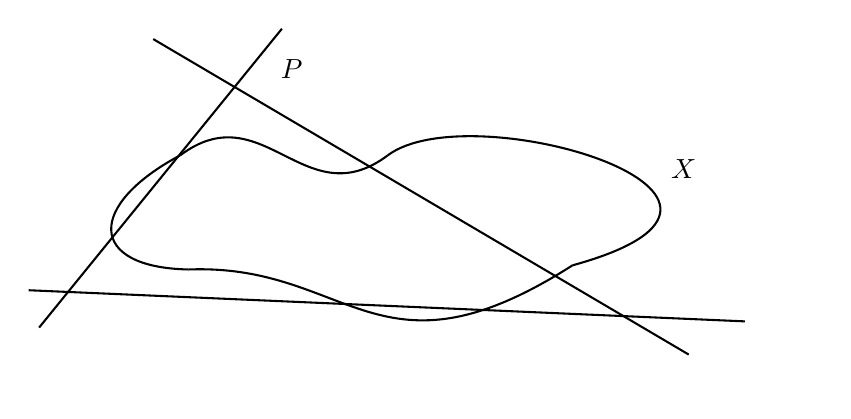
\begin{tikzpicture}[
            x=0.75pt,
            y=0.75pt,
            yscale=-1,
            xscale=1,
            every node/.style={text=black},
            every path/.style={draw=black},
            line width=0.75pt
        ]
    %uncomment if require: \path (0,300); %set diagram left start at 0, and has height of 300

    %Curve Lines [id:da5176716541451285]
            \draw    (171,91) .. controls (211,61) and (231,121) .. (271,91) ;
    %Curve Lines [id:da11034559807114497]
            \draw    (271,91) .. controls (311,61) and (480,111) .. (360,144) ;
    %Curve Lines [id:da21598744094903344]
            \draw    (175,146) .. controls (253,143) and (266,204) .. (360,144) ;
    %Curve Lines [id:da06058426431395958]
            \draw    (175,146) .. controls (126,145) and (126,115) .. (171,91) ;
    %Straight Lines [id:da11549073425210676]
            \draw    (158,35) -- (416,187) ;
    %Straight Lines [id:da0608839383942672]
            \draw    (220,30) -- (103,174) ;
    %Straight Lines [id:da2736385464060678]
            \draw    (98,156) -- (443,171) ;

    % Text Node
            \draw (189,52.4) node [anchor=north west][inner sep=0.75pt]  [font=\scriptsize]  {$\CIRCLE $};
    % Text Node
            \draw (406,91.4) node [anchor=north west][inner sep=0.75pt]    {$X$};
    % Text Node
            \draw (218,43.4) node [anchor=north west][inner sep=0.75pt]    {$P$};


        \end{tikzpicture}
    }
    \caption{Because $\pp^2\setminus\{U\cup V\} = p$}
\end{figure}
We can always choose $X$ to avoid this point. So, $\div(\omega) = 0$ on $U$ and $\div(\omega) = (d-3)D$ on $V$. Thus $\div(\omega) = (d-3)D$ on $X$ is a canonical divisor of class $K_X$.\\ \\
The degree of $K_X$ is $\deg(K_X) = d(d-3)$. If $d = 1$ meaning $X\cong\pp^1$ line, then $\deg(K_x) = -2$. If $d = 2$ meaning $X\cong \pp^1$ a smooth conic, then $\deg(K_X) = 2(-1) = -2$.
